\PassOptionsToPackage{unicode=true}{hyperref} % options for packages loaded elsewhere
\PassOptionsToPackage{hyphens}{url}
%
\documentclass[]{article}
\usepackage{lmodern}
\usepackage{amssymb,amsmath}
\usepackage{ifxetex,ifluatex}
\usepackage{fixltx2e} % provides \textsubscript
\ifnum 0\ifxetex 1\fi\ifluatex 1\fi=0 % if pdftex
  \usepackage[T1]{fontenc}
  \usepackage[utf8]{inputenc}
  \usepackage{textcomp} % provides euro and other symbols
\else % if luatex or xelatex
  \usepackage{unicode-math}
  \defaultfontfeatures{Ligatures=TeX,Scale=MatchLowercase}
\fi
% use upquote if available, for straight quotes in verbatim environments
\IfFileExists{upquote.sty}{\usepackage{upquote}}{}
% use microtype if available
\IfFileExists{microtype.sty}{%
\usepackage[]{microtype}
\UseMicrotypeSet[protrusion]{basicmath} % disable protrusion for tt fonts
}{}
\IfFileExists{parskip.sty}{%
\usepackage{parskip}
}{% else
\setlength{\parindent}{0pt}
\setlength{\parskip}{6pt plus 2pt minus 1pt}
}
\usepackage{hyperref}
\hypersetup{
            pdftitle={Final Project},
            pdfauthor={Yihao Zhang},
            pdfborder={0 0 0},
            breaklinks=true}
\urlstyle{same}  % don't use monospace font for urls
\usepackage[margin=1in]{geometry}
\usepackage{graphicx,grffile}
\makeatletter
\def\maxwidth{\ifdim\Gin@nat@width>\linewidth\linewidth\else\Gin@nat@width\fi}
\def\maxheight{\ifdim\Gin@nat@height>\textheight\textheight\else\Gin@nat@height\fi}
\makeatother
% Scale images if necessary, so that they will not overflow the page
% margins by default, and it is still possible to overwrite the defaults
% using explicit options in \includegraphics[width, height, ...]{}
\setkeys{Gin}{width=\maxwidth,height=\maxheight,keepaspectratio}
\setlength{\emergencystretch}{3em}  % prevent overfull lines
\providecommand{\tightlist}{%
  \setlength{\itemsep}{0pt}\setlength{\parskip}{0pt}}
\setcounter{secnumdepth}{0}
% Redefines (sub)paragraphs to behave more like sections
\ifx\paragraph\undefined\else
\let\oldparagraph\paragraph
\renewcommand{\paragraph}[1]{\oldparagraph{#1}\mbox{}}
\fi
\ifx\subparagraph\undefined\else
\let\oldsubparagraph\subparagraph
\renewcommand{\subparagraph}[1]{\oldsubparagraph{#1}\mbox{}}
\fi

% set default figure placement to htbp
\makeatletter
\def\fps@figure{htbp}
\makeatother

\usepackage{booktabs}
\usepackage{longtable}
\usepackage{array}
\usepackage{multirow}
\usepackage{wrapfig}
\usepackage{float}
\usepackage{colortbl}
\usepackage{pdflscape}
\usepackage{tabu}
\usepackage{threeparttable}
\usepackage{threeparttablex}
\usepackage[normalem]{ulem}
\usepackage{makecell}
\usepackage{xcolor}

\title{Final Project}
\author{Yihao Zhang}
\date{4/30/2020}

\begin{document}
\maketitle

\textbf{Introduction}

Due to the outbreak of COVID-19 as a global pandemic, oil storage
facilities were reaching their limits. On April 20, 2020, U.S. crude oil
prices dropped by almost 300 percent to turn negative for the first time
in history and reach negative \$37.63 a barrel.

Retail gasoline is a consumer product that is refined from crude oil and
its closely related to our daily life. It is a complementary good of
motor vehicles, which is one of the main tools for people's daily
transportation. The recent dramatical fluctuations of crude oil prices
have affected the price of retail gasoline, and this brought the
interest in analyzing how people's travel behavior responses to the
fluctuations of gasoline prices. Will an increase in retail gasoline
price affect people's travel behavior by increasing regional demand on
public transportation as an effort to reduce travel expenditure? If so,
a comprehensive understanding of how people's demand for public
transportation changes in response to a change in gasoline price can
provide an important guideline to public transit agencies on capacity
management and pricing strategy during a period when gasoline price
fluctuates.

Based on this scope, this analysis will use the panel data of public
transportation ridership and retail gasoline price from the Austin area
from 2016 to 2020 along with a control group of specific factors to
estimate the short-run effect of change in gasoline prices on transit
ridership.

\textbf{Methodology}

This analysis used both static linear regression model and a dynamic
regression model for metro ridership estimation. The first model
estimated the contemporaneous relationship of metro ridership and
relevant external variables, and the second model takes both the effect
of past observations on metro ridership and relevant external variables
to improve the forecast accuracy. The aim here is to estimate the
elasticity of metro ridership to gasoline price and to specify; this
study is predicting the percentage change in metro ridership in response
to one percentage change in retail gasoline price.

Table 1 illustrates the information of dependent and independent
variables included in both regression analysis as well as the source of
data. The range of the data site for all variables is from October 2016
to February 2020 monthly.

\begin{table}[H]
\centering
\begin{tabular}{>{\bfseries}l||l|l|l}
\hline
\multicolumn{4}{c|}{Table 1: Dependent and Independent Variables Used in Studies as well as Their Specifications. } \\
\cline{1-4}
Variable & Feature & Description & Source\\
\hline
Metro Ridership & Dependent Variable & Measured the sum of Monthly ridership with MetroAccess, MetroBus, MetroExpress, MetroRail and MetroRapid in Austin City, implemented log transformation afterwards. & U.S. Energy Information administration\\
\hline
Retail Gasoline price & Independent Variable & Used Texas regular conventional retail gasoline price to represent the gasoline price in Austin City. Raw Data acquired is in Weekly basic, transformed into average monthly data, implemented log transformation afterwards. & Capital Metropolitan Transportation Authority\\
\hline
Temperature & Independent Variable & Measured the monthly average temperature (Fahrenheit) in Austin City, implemented log transformation afterwards. & National Weather Service Forecast\\
\hline
Precipitation & Independent Variable & Measured the monthly total precipitation in inch in Austin City, implemented log transformation afterwards. & National Weather Service Forecast\\
\hline
Unemployment & Independent Variable & Measured the monthly unemployment rate in Austin City. & The Bureau of Labor Statistics\\
\hline
\end{tabular}
\end{table}

As seen in Table 1, in addition to Metro Ridership and Retail Gasoline
Price, Temperature, Precipitation, and unemployment rate have been
considered as explanatory variables. Temperature and Precipitation are
weather indicators that can strongly affect people's travel behavior. In
mild sunny days, more people will be more willing to walk to and from
their destinations while on rainy days, more people will prefer to take
public transportations. Unemployment is another substantial explanatory
variable; a lower unemployment rate means there will be more people who
have chances to take the metro to work.

Besides these 4 explanatory variables, serval other external variables
have been considered to involve in the study and were dropped out later.
These variables include metro fare, average household income, and metro
service rating. Metro fare and average household income were dropped
from the study because both variables remain stable from 2016-2020 every
month. Metro service rating has not been considered due to the
non-existence of an official data report.

The following sub-sections describe the regression modeling process
within the framework of both static data and panel data analysis for
transit ridership estimation.

\textbf{Static Regression Model}

Here, we are modeling a contemporaneous relationship between Metro
Ridership and other independent variables with the assumption that the
change among the independent variables will have an immediate effect on
the dependent variable (metro ridership).

Before building the prediction model, the whole dataset was separated
into a training group and a testing group. The training group counts for
80\% of the observations recorded from October 2016 to May 2019, and the
testing group counts for the rest 20\% observations, which is from June
2019 to February 2020.

Next, two-way interaction automatically iterative model selection method
is implemented for our model selection. Given the result, models
generated from forwarding Selection and Stepwise Selection provided the
same information criteria.

\begin{itemize}
\tightlist
\item
  Model1 : log(\(y\)) = 14.350 + 0.142log(\({x_1}\))
  +0.058log(\({x_2}\)) -0.006log(\({x_3}\)), AIC = -152.42
\item
  Model2 : log(\(y\)) = 14.507 - 0.045log(\({x_1}\))
  +0.123log(\({x_2}\)) -0.008log(\({x_3}\)) - log(\({x_4}\)), AIC =
  -152.42
\end{itemize}

Then, out-of-sample estimation accuracy was computed, and the result is
in table 2.

\begin{table}[H]
\centering
\begin{tabular}{>{\bfseries}l||r|r}
\hline
\multicolumn{3}{c|}{Table 2: Out of Sample Prediction Accuracy  } \\
\cline{1-3}
  & MAPE & RMSE\\
\hline
Model 1 & 0.5063061 & 0.0973204\\
\hline
Model 2 & 0.4271024 & 0.0795031\\
\hline
\end{tabular}
\end{table}

As seen in Table 2, Model 1 made a better out of sample accuracy
performance; it generated a lower RMSE and MAPE. We can conclude that
Model 1 is our best static regression model for metro ridership
estimation.

Dynamic Regression Model

Figure 1 shows the relationship between metro ridership - representing
the sum of ridership with MetroAccess, MetroBus, MetroExpress,
MetroRail, and MetroRapid and average retail gasoline prices in Austin
City.

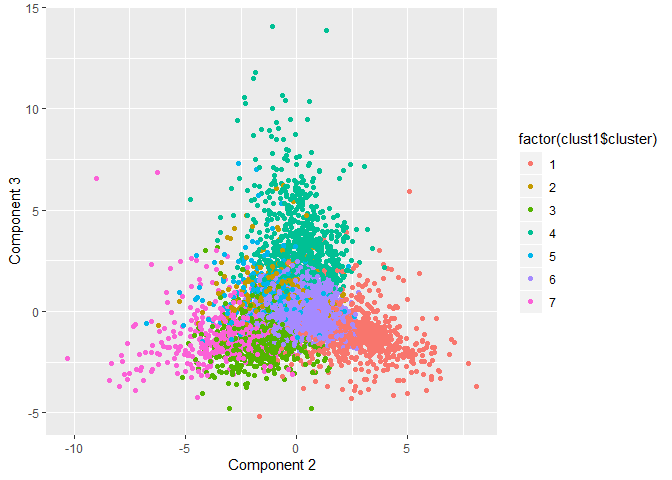
\includegraphics{report_files/figure-latex/unnamed-chunk-6-1.pdf}

These two variables follow a similar trend pattern during a certain
period. Furthermore, in fact, due to information asymmetry, it is
reasonable to suggest that the effect of the gasoline price change on
ridership is inherently temporal since people will not be notified
simultaneously when the gasoline price changes. So, here we are going to
perform a dynamic regression analysis to examining temporal and lagged
effects of changes in variables.

Here we have equation 1 which express the specification that the model I
will fit using panel data with a group of control variables.

\({Y_{t}}\) = \({a_0}\) + \({B}\)\({X_{t}}\) + \({n_t}\) +
\(\epsilon_{t}\) equation 1

where

\({Y_{it}}\) denotes metro ridership in Austin area at time t.

\({a_0}\) denotes the intercept parameter.

\({B}\) are vector of slope parameters associated with external
influential factors.

\({X_t}\) is the vector of external influential factors that include
gasoline price, average temperature, total precipitation, unemployment
rate in Austin area at time t.

\({n_t}\) denotes monthly fixed effects to represent seasonal variation
in transit ridership.

\(\epsilon_{t}\) denotes the stochastic error term corresponding to the
regression for the mode.

\end{document}
